documentclass{article}
\usepackage{tikz}
\usetikzlibrary{positioning,fit,backgrounds,calc,tikzmark}
\usepackage{xcolor}

\begin{document}

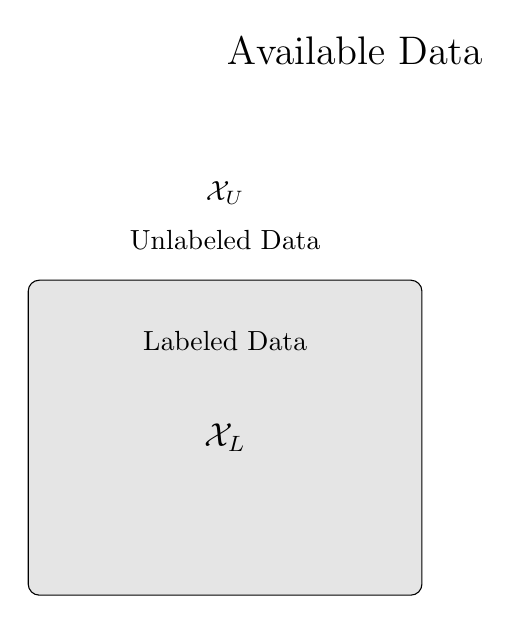
\begin{tikzpicture}[node distance = 10mm]
    \node (unlabeled) [rectangle, rounded corners, draw=black, fill=gray!20, minimum width=5cm,minimum height=4cm,label={[anchor=north,yshift=-1.5em]north:Labeled Data}] {\large{$\mathcal{X}_{L}$}};
    \node (labeled) [above right =of unlabeled.north west,xshift=1.7cm,yshift=1.9cm] {\Large{Available Data}};
    \node (unlabelednode) [anchor=center] at ($(unlabeled.north)+(0,.5cm)$) {Unlabeled Data};
    \node (unlabelednode2) [anchor=center] at ($(unlabelednode)+(0,.6cm)$) {$\mathcal{X}_U$};
    \end{tikzpicture}

\end{document}